\documentclass[12pt]{article}
\usepackage{fancyhdr,epsfig,graphics,tabularx,times}
\pagestyle{empty}
\topmargin=-0.75in
\oddsidemargin=-0.5in
\textwidth=7.5in
\textheight=10.25in
\parindent=0.0in
\parskip=10pt
\linespread{1.0}

\renewcommand{\labelenumi}{(\alph{enumi})}
\renewcommand{\thefigure}{\arabic{section}.\arabic{figure}}
\def\thesection{Problem \#\arabic{section}}

\begin{document}
{\bf BME154L - Spring 2012 - Exam \#2 Solutions}\hfill Name (Net ID):\underline{\hspace*{3.0in}}



\vspace*{0.5in}

\centerline{\LARGE BME354L (Palmeri)}
\vspace*{0.25in}
\centerline{\LARGE Spring 2013}
\vspace*{0.25in}
\centerline{\LARGE Exam \#2}
\vspace*{0.25in}

{\bf Instructions:} 
\begin{itemize}
\item Write your name at the top of each page.
\item {\bf Show all work (this is {\it critical} for partial credit!)}.
\item Remember to include units with all answers and label all plot axes.
\item Clearly delineate all answers.
\item Assume that all components are ideal unless otherwise stated.
%\item Assume that op amps rail at $\pm$ 12 V unless otherwise stated.
\item Please keep your answers brief for questions where I ask `why?'.
\end{itemize}

\vspace*{3in}

\emph{In keeping with the Duke Community Standard, I have neither given nor received aid in completion of this examination.}

\vspace*{0.5in}

Signature:\underline{\hspace*{3.0in}}


\clearpage

{\bf BME154L - Spring 2012 - Exam \#2 Solutions}\hfill Name (Net ID):\underline{\hspace*{3.0in}}



%\section{[10 points]}
%
%Given $V_1(t)$ = 0.1 cos(200$\pi t$ + $\frac{\pi}{8}$) and $V_2(t)$ = 0.5 cos(200000$\pi t$
%+ $\pi$) V, $R_1$ = 10 k$\Omega$, $R_2$ = 20 k$\Omega$ and $C_1$ = 8 nF, sketch
%several cycles of $V_o(t)$.
%
%\begin{center}
%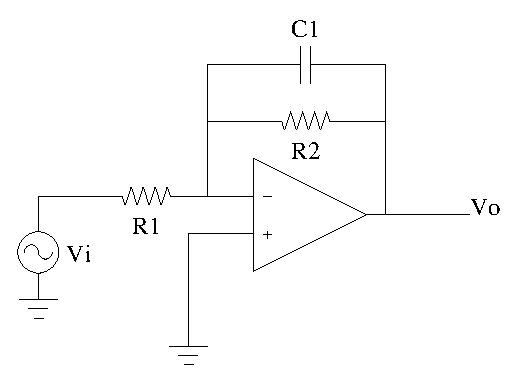
\includegraphics[width=0.4\linewidth]{active_lpf.eps}
%\end{center}
%
%\clearpage
%
%{\bf BME154L - Spring 2012 - Exam \#2 Solutions}\hfill Name (Net ID):\underline{\hspace*{3.0in}}


%
%\section{[10 points]}
%
%Given $V_i(t)$ = 0.1 cos(200$\pi t$ + $\frac{\pi}{8}$) + 0.5 cos(200000$\pi t$
%+ $\pi$) V, $R_1$ = 20 k$\Omega$ and $C_1$ = 8 nF, sketch several cycles of
%$V_C(t)$ and $V_R(t)$.
%
%\begin{center}
%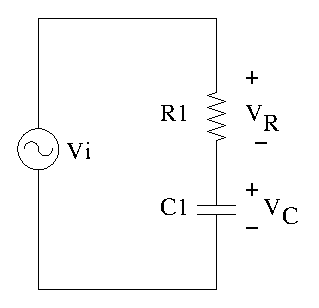
\includegraphics[width=0.3\linewidth]{passive_filt.eps}
%\end{center}
%
%\clearpage
%
%{\bf BME154L - Spring 2012 - Exam \#2 Solutions}\hfill Name (Net ID):\underline{\hspace*{3.0in}}


%
\section{[45 points]}

Given $V_i(t)$ = 0.050 + 0.1 cos(200$\pi t$) + 0.5 sin(2000000$\pi t$) V and the
threshold voltage for the diodes is 0.7 V:

\begin{center}
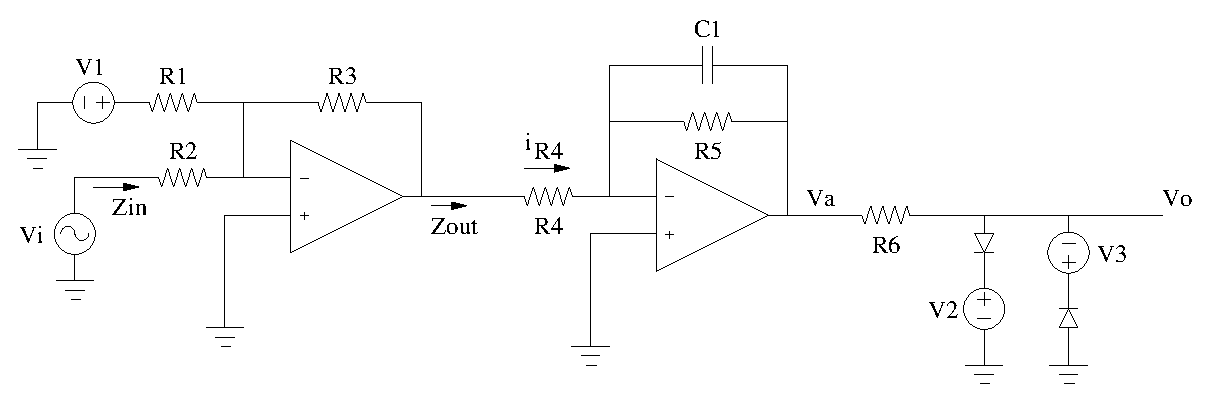
\includegraphics[width=1.0\linewidth]{sum_filt_comp.eps}
\end{center}

\begin{enumerate}
\item What is $Z_{in}$ (in terms of symbolic values)?  (as indicated on the circuit schematic)
\item What happens to $Z_{in}$ if $R_3$ is twice as large (2$R_3$)?
\item Assign values to the necessary components in the circuit such that $V_a(t)$:
\begin{enumerate}
\item[1.] has the 50 mV DC offset voltage from $V_i(t)$ removed, 
\item[2.] has the 1000000 Hz component of $V_i(t)$ attenuated by at least 40 dB from
the 100 Hz signal component while minimizing the phase distortion of the 100 Hz
signal component, and, 
\item[3.] has the peak-to-peak voltage of the 100 Hz signal component amplified to
$\pm$ 2V. 
\end{enumerate}
Write an expression for $V_a(t)$.
\item Given the circuit element values that you have chosen, what is $Z_{out}$?  (as indicated on the circuit schematic)
\item What happens to $Z_{out}$ if $R_4$ is twice as large (2$R_4$)?
\item Write an expression for $i_{R_4}$?  (Reality check: can a op amp generate that amount of current?)
\item If $V_2$ = 0.5 V, $V_3$ = 0.25 V, and $R_6$ = 1 k$\Omega$, then sketch
several cycles of $V_o(t)$.
\item What happens to your above sketch of $V_o(t)$ if $R_6$ = 10 k$\Omega$?
\end{enumerate}

\clearpage

{\bf BME154L - Spring 2012 - Exam \#2 Solutions}\hfill Name (Net ID):\underline{\hspace*{3.0in}}



\clearpage

{\bf BME154L - Spring 2012 - Exam \#2 Solutions}\hfill Name (Net ID):\underline{\hspace*{3.0in}}



\clearpage

{\bf BME154L - Spring 2012 - Exam \#2 Solutions}\hfill Name (Net ID):\underline{\hspace*{3.0in}}



\section{[25 points]}

An electroencephalogram (EEG) contains biosignals that range from 1 Hz - 10
MHz.  A researcher in the neurosciences wants to isolate two distinct frequency
bands: (1) 1 - 100 Hz and (2) 100 kHz - 100 MHz.  The lower frequency signals are
very weak ($\sim$20 mV peak-to-peak), while the higher frequency signals are
slightly stronger ($\sim$100 mV peak-to-peak).  Design a circuit that:
\begin{enumerate}
\item [1.] suppresses white noise outside the desired signal frequency bands as
best as possible (100 Hz - 100 kHz and $>$100 MHz), and 
\item [2.] generates an output signal that contains both desired signal
frequency bands, with $\sim$500 mV peak-to-peak signal amplitude for both
frequency bands.  
\end{enumerate}
The phase of the preserved signals should be distorted as little as possible.

\clearpage

{\bf BME154L - Spring 2012 - Exam \#2 Solutions}\hfill Name (Net ID):\underline{\hspace*{3.0in}}



\clearpage

{\bf BME154L - Spring 2012 - Exam \#2 Solutions}\hfill Name (Net ID):\underline{\hspace*{3.0in}}



\section{[30 points]}

A pulmonary artery catheter is equipped with a thermistor to measure the
temperature of blood being pumped to the lungs from the heart.  A patient is
given an intravenous bolus of cold saline that drops the temperature of blood
in their pulmonary artery linearly from 27 $^\circ$C to 22 $^\circ$C over a
period of 30 seconds after the injection.  The thermistor has a resistance of
100 $\Omega$ at 27 $^\circ$C, and its resistance linearly varies as a function
of temperature by 1 $\pm$ 0.05 $\Omega$/$^\circ$C.  Design a circuit that
converts the thermistor's resistance change into a voltage signal, and
illuminates an LED when the temperature drops below 25 $^\circ$C in the
pulmonary artery during the 30 second injection.  Make your circuit robust
enough so that the LED does not ``flicker'' due to variability in the
thermistor's resistance as a function of temperature.

\clearpage

{\bf BME154L - Spring 2012 - Exam \#2 Solutions}\hfill Name (Net ID):\underline{\hspace*{3.0in}}



\end{document}
